\documentclass[a0paper,portrait]{baposter}



\usepackage{wrapfig}
\usepackage{lmodern}

\usepackage[utf8]{inputenc} %unicode support
\usepackage[T1]{fontenc}

\usepackage{tikz}
\usetikzlibrary{bayesnet}

\selectcolormodel{cmyk}

\graphicspath{{figures/}} % Directory in which figures are stored


%%%%%% math commands


\usepackage{amsmath,amsfonts,amssymb,amsthm}

\usepackage{bm}
\usepackage{hyperref}

\newcommand{\tr}{\intercal}
\newcommand{\eye}{\mathrm{I}}
\newcommand\given[1][]{\:#1\vert\:}

\newcommand{\transpose}[1]{#1^{\intercal}}
\newcommand{\R}{\mathbb{R}}
\newcommand{\nprod}{\prod\limits_{n}}
\newcommand{\kprod}{\prod\limits_{k}}
\newcommand{\nsum}{\sum\limits_{n}}
\newcommand{\ksum}{\sum\limits_{k}}
\newcommand{\boldbeta}{\boldsymbol\beta}
\newcommand{\boldgamma}{\boldsymbol\gamma}
\newcommand{\boldtau}{\boldsymbol\tau}
\newcommand{\sumexp}{\sum_{j=1}^{K} e^{ \transpose{x_n} \gamma_j}}
\newcommand{\E}{\mathbb{E}}
\newcommand{\diagdots}{_{^{\big\cdot}\cdot _{\big\cdot}}}
% \newcommand{\var}{\mathrm{Var}}

\newcommand{\betad}{\tilde{\beta}_d}
\newcommand{\betaj}{\tilde{\beta}_j}
\newcommand{\umat}{\mathrm{U}}
\newcommand{\qmat}{\mathrm{Q}}

\newcommand{\priorbeta}{\mathcal{N} \left( \betad \given 0, \xi_0^{-1} \cdot \mathrm{I}_K \right)}
\newcommand{\qbeta}{\mathcal{N} \left( \betad \given m_d, \qmat_d^{-1} \right)}


\usepackage{setspace}
\let\Algorithm\algorithm
\renewcommand\algorithm[1][]{\Algorithm[#1]\setstretch{1.05}}


\newcommand{\pr}[1]{p \left( #1 \right)}
\newcommand{\trace}[1]{\mathrm{tr} \left( #1 \right)}
\newcommand{\var}[1]{\mathrm{Var}\left(#1\right)}

%%%%%% math commands



\newcommand{\compresslist}{%
\setlength{\itemsep}{0pt}%
\setlength{\parskip}{1pt}%
\setlength{\parsep}{0pt}%
}

\newenvironment{boenumerate}
  {\begin{enumerate}\renewcommand\labelenumi{\textbf\theenumi.}}
  {\end{enumerate}}



\begin{document}


%\definecolor{darkgreen}{cmyk}{0.8,0,0.8,0.45}
\definecolor{darkgreen}{cmyk}{0.52, 0.25, 0, 0.66}
\definecolor{lightgreen}{cmyk}{0.52, 0.25, 0, 0.35}

\begin{poster}
{
grid=false,
headerborder=open, % Adds a border around the header of content boxes
colspacing=1em, % Column spacing
bgColorOne=white, % Background color for the gradient on the left side of the poster
bgColorTwo=white, % Background color for the gradient on the right side of the poster
borderColor=darkgreen, % Border color
headerColorOne=lightgreen, % Background color for the header in the content boxes (left side)
headerColorTwo=lightgreen, % Background color for the header in the content boxes (right side)
headerFontColor=white, % Text color for the header text in the content boxes
boxColorOne=white, % Background color of the content boxes
textborder=rounded, %rectangle, % Format of the border around content boxes, can be: none, bars, coils, triangles, rectangle, rounded, roundedsmall, roundedright or faded
eyecatcher=false, % Set to false for ignoring the left logo in the title and move the title left
headerheight=0.11\textheight, % Height of the header
headershape=rounded, % Specify the rounded corner in the content box headers, can be: rectangle, small-rounded, roundedright, roundedleft or rounded
headershade=plain,
headerfont=\Large\textsf, % Large, bold and sans serif font in the headers of content boxes
%textfont={\setlength{\parindent}{1.5em}}, % Uncomment for paragraph indentation
linewidth=2pt % Width of the border lines around content boxes
}
{}
%
%----------------------------------------------------------------------------------------
%	TITLE AND AUTHOR NAME
%----------------------------------------------------------------------------------------
%
{
\textsf %Sans Serif
{Variational Inference for Bayesian Density Regression.
}
} % Poster title
% {\vspace{1em} Marta Stepniewska, Pawel Siedlecki\\ % Author names
% {\small \vspace{0.7em} Department of Bioinformatics, Institute of Biochemistry and Biophysics, PAS, Warsaw, Pawinskiego 5a}} % Author email addresses
{\sf\vspace{0.5em}\\
Eric Chuu
\vspace{0.1em}\\
\small{Department of Statistics, Texas A&M University
\vspace{0.2em}\\
ericchuu@tamu.edu}
}
% {
\includegraphics{logo}} % University/lab logo


\headerbox{1. Introduction}{name=introduction,column=0,row=0, span=2}{
In the Bayesian density regression problem, we observe data $\left(y_n, x_n \right), n=1, \ldots, N$, and the goal is the estimate the conditional density of $y \given x$. A common approach for doing this is to model the density using a mixture of Gaussians. We extend this idea by allowing the covariates to enter the weights through a logit link function.
\begin{equation*}
	 f(y \given x) = \sum_{k}^{K} \pi_k(x) \cdot \mathcal{N} \left( y \given \mu_k(x), \tau_k^{-1} \right) 
\end{equation*} 
where $\mu_k(x) = \transpose{x} \beta_k$ and $\pi_{k}(x) \propto \exp(\transpose{x} \gamma_k)$. While this increases the flexibility of the model, it also increases the computational complexity. In order to perform fast inference on the model parameters, we adopt a variational approach to obtain an approximating distribution to the true posterior. This setup, however, requires an approximation of the softmax function to achieve closed form updates for the coordinate ascent algorithm. We demonstrate the algorithm on both synthetic and real datasets, and we consider extensions of the algorithm via variable selection. \\

\vspace{3pt}
}

\headerbox{2. Notation}{name=notation,column=2,row=0, span=1}{
\begin{itemize} \setlength\itemsep{0.07em}
	\item Data: $\mathbf{y} = \{y_{1:N} \}, \mathbf{X} = \{ x_{1:N} \} \subseteq \R^{D}$
	\item Coefficient Vector (Gaussian): $\boldbeta = \{ \beta_{1:K} \}$ 
	\item Precision (Gaussian): $\boldtau = \{ \tau_{1:K} \}$
	\item Coefficient Vector (weights): $\boldgamma = \{ \gamma_{1:K} \}$
	\item Cluster Indicator: $\mathbf{Z} = \{ z_{1:N} \} \subseteq \R^K$
\end{itemize}
  \begin{center}
  \tikz{ %
    \node[latent] (gamma) {$\gamma$} ; %
    \node[latent, right=of gamma] (z) {$z_n$} ; %
    \node[obs, right=of z] (yn) {$y_n$} ; %
    \node[det, below =of yn] (xn) {$x_n$};
    \node[latent, right=of xn] (tau) {$\tau$} ; %
    \node[latent, right=of yn] (beta) {$\beta$} ; %
    \plate[inner sep=0.2cm, xshift=-0.12cm, yshift=0.05cm] {plate1} {(z) (yn) (xn)} {N}; %
    \edge {gamma} {z} ; %
    \edge {z,tau,beta} {yn} ; %
    \edge {beta} {yn} ; %
    \edge {tau} {beta} ; %
    \edge {xn} {yn}
    \edge {xn} {z}
  }
  \end{center}
}


\headerbox{3. Model Setup}{name=model,column=0,below=introduction,span=1}{

Introducing the cluster indicators, we can simplify the conditional density. In addition, we consider conjugate priors to ease computation. 
\begin{align*}
	p \left( \mathbf{y} \given \mathbf{X}, \boldsymbol\beta, \boldsymbol{\tau}, \mathbf{Z} \right) &= 
	\prod_{n} \prod_{k} \mathcal{N} \left( y_n \given \transpose{x_n} \beta_k, \tau_{k}^{-1} \right)^{z_{nk}} \\
	p \left( \mathbf{Z} \given \mathbf{X}, \boldsymbol\gamma \right) &= 
	\nprod \kprod \Bigg[ \frac{e^{\transpose{x_n} \gamma_k}}{\sumexp}\Bigg]^{z_{nk}} \\
	p \left( \boldgamma \right) &= \prod_{k} \mathcal{N} \left( \gamma_k \given 0, \eye_{D} \right) \\
	p \left( \boldbeta, \boldtau \right) &= \prod_{k} p \left(\beta_k \given \tau_k \right) p\left(\tau_k\right) \\
	p \left( \beta_k\given \tau_k \right) &= \mathcal{N} \left( \beta_k \given m_0, \left(\tau_k \Lambda_0\right)^{-1} \right) \\
	p\left(\tau_k \right) &= \mathrm{Gamma} \left( \tau_k \given a_0, b_0 \right)
\end{align*}



}


\headerbox{3. Variational Approximation}{name=variational,column=1,below=notation,span=2}{

To measure similarity of two molecules or to combine them into one model, DeCAF first finds their \textbf{maximum common substructure (MCS)}.
To provide fast, but accurate method for solving MCS problem, we combined Generic Match Algorithm (GMA) \cite{xu1996gma} with backtracking algorithm proposed by Yiqun Cao \cite{cao2008maximum}.

Here we present comparison of molecules with similar and with different structures.
DeCAF scores and \textbf{Tanimoto coefficient (Tc)} values are shown in red and black, respectively.


}

\headerbox{4. Application to Bimodal Conditional Densities}{name=screen,span=2,column=1,below=variational}{ % To reduce this block to 1 column width, remove 'span=2'

DeCAF is a versatile tool with many possible applications.
It allows to compare two molecules or more complex models created from sets of ligands.
Our method can be used to align multiple ligands and find crucial pharmacophoric features in a set of active compounds.
Pharmacophore models can help in database screening for molecules with desired properties.
DeCAF is also suitable for comparing entire sets of ligands, e.g. to analyse properties of proteins in drug repositioning process. DeCAF is a versatile tool with many possible applications.
It allows to compare two molecules or more complex models created from sets of ligands.
Our method can be used to align multiple ligands and find crucial pharmacophoric features in a set of active compounds.
Pharmacophore models can help in database screening for molecules with desired properties.
DeCAF is also suitable for comparing entire sets of ligands, e.g. to analyse properties of proteins in drug repositioning process.

% \vspace{-5pt}


}


\headerbox{5. Application to Speedflow Data}{name=sea,span=2,column=1,below=screen}{ % To reduce this block to 1 column width, remove 'span=2'

\begin{wrapfigure}{l}{0.3\textwidth}
    \vspace{10pt}
    \begin{center}
        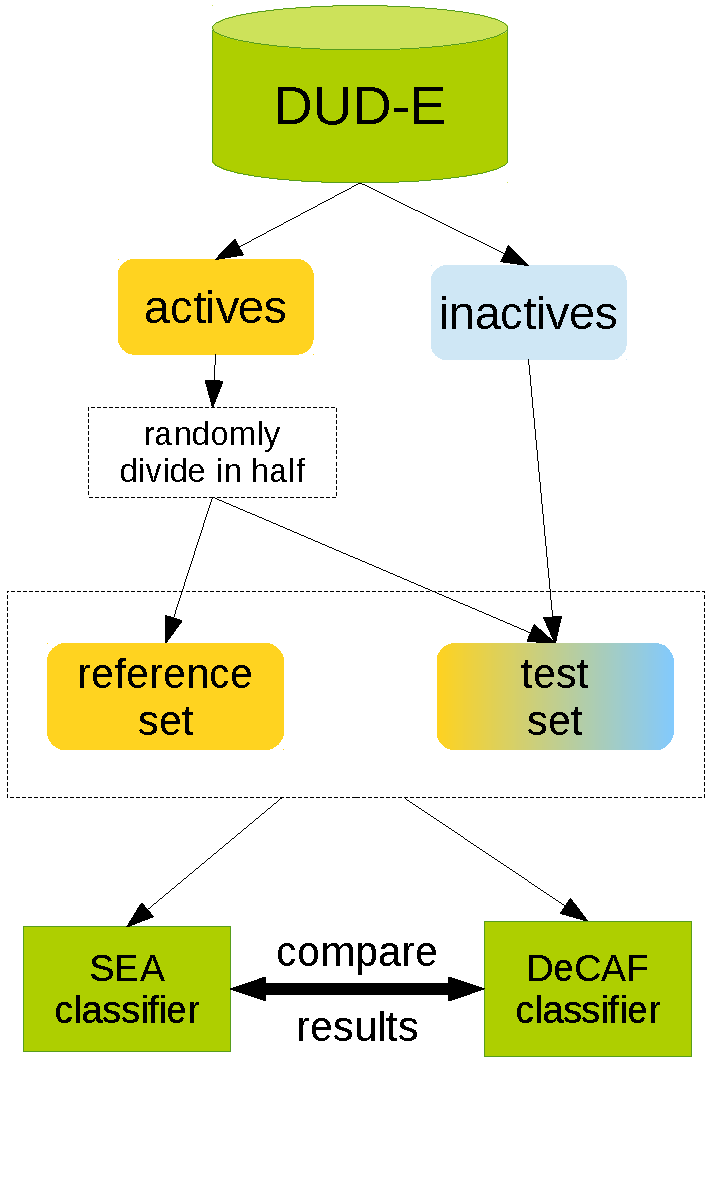
\includegraphics[width=\linewidth]{class}
    \end{center}
    %\vspace{-145pt}
\end{wrapfigure}

We examine the results of this algorithm applied to both synthetic datasets and a real dataset involving the distribution of speed for different traffic flows on one of California's freeways. We examine the results of this algorithm applied to both synthetic datasets and a real dataset involving the distribution of speed for different traffic flows on one of California's freeways. We examine the results of this algorithm applied to both synthetic datasets and a real dataset involving the distribution of speed for different traffic flows on one of California's freeways. We examine the results of this algorithm applied to both synthetic datasets and a real dataset involving the distribution of speed for different traffic flows on one of California's freeways. 

\hspace{0pt}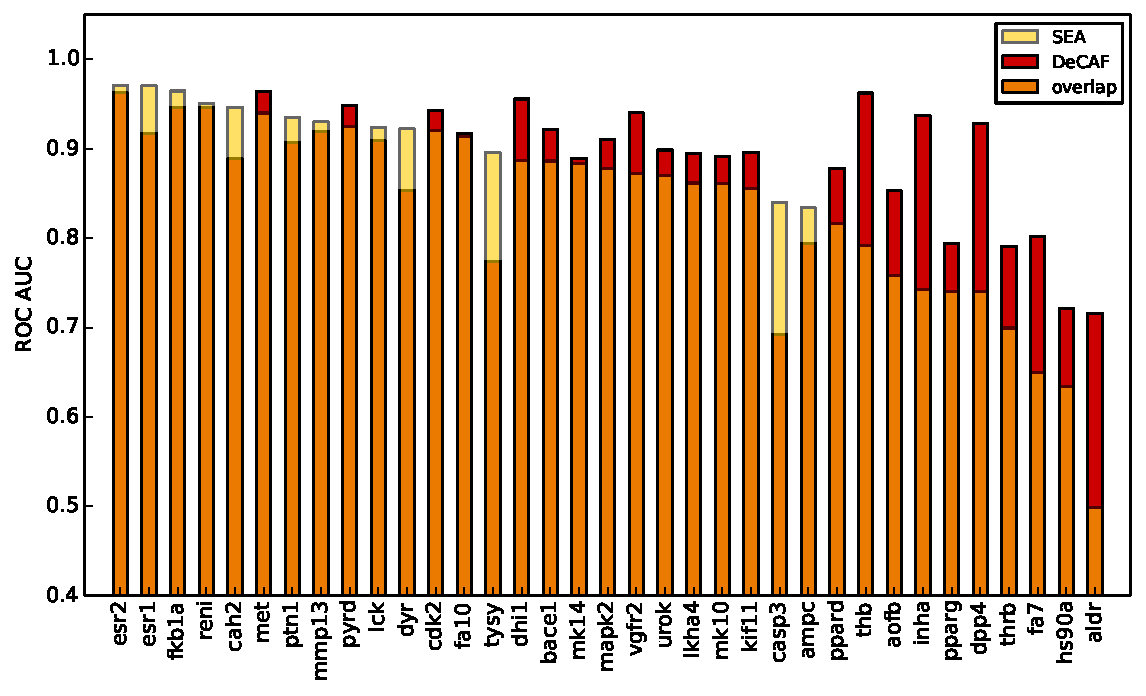
\includegraphics[width=0.95\linewidth]{res}

}


%\headerbox{6. Extension of Algorithm via Variable Selection}{name=conclusion,column=1,below=sea,span=2,above=bottom}{
% DeCAF is a chemoinformatical tool that can be helpful in ligand-based drug design.
% It provides a comprehensive molecule description and a fast algorithms for comparing and aligning multiple ligands.
%We proved that DeCAF is a significant improvement over the SEA algorithm, a popular method for comparing sets of ligands.
%\begin{boenumerate}\compresslist
%    \item DeCAF gives better results for 23 out of 35 receptors.
%    \item For targets with easily separable active and inactive datasets, SEA and DeCAF give similar results.
%    \item In cases in which SEA fails to identify active molecules, our method performs substantially better.
%\end{boenumerate}
% It can be also used in other [procedures], such as database screening or drug repositioning.
% DeCAF is written in Python and freely available at \textbf{\color{darkgreen}http://bitbucket.org/marta-sd/decaf}. 
%}


\headerbox{6. Variable Selection}{name=vs,column=0,span=1,below=model,above=bottom}{

%\small % Reduce the font size in this block
\renewcommand{\section}[2]{\vskip 0.05em} % Get rid of the default "References" section title
%\nocite{*} % Insert publications even if they are not cited in the poster





\bibliographystyle{unsrt}
\bibliography{poster} % Use sample.bib as the bibliography file
}

\end{poster}

\end{document}
